\subsubsection{Proportional Integral and Derivative (PID) Control}\label{sec:pid}

In 1922, Nicolas Minorsky presented a very clear analysis of the control actions necessary to provide effective control of a system whose exact dynamics were un- known. He analyzed the actions taken by a good helmsman steering a ship and translated these actions into the appropriate mathematical formulations \parencite{bennett1993pid}. It is now know as the Proportional-Integral-Derivative (PID) controller. PID is a type of controller that is most commonly used and applied in mechanical systems \parencite{idrissi_review_2022}. Also used in many modern quadcopters, PID is employed here to stabilize drone movement and to function as a trainer AI.

The controller consists of three main components: Proportional ($K_p$): Acts like a virtual spring that pulls the system toward the desired position; the control action increases as the error gets larger; Integral ($K_i$): Accumulates the error over time to eliminate steady-state error, ensuring the drone reaches the exact target even in the presence of disturbances like gravity; Derivative ($K_d$): Acts as a virtual damper to reduce oscillations and prevent the system from overshooting its target.

The idealized control law is expressed as \cref{eq:pid}.

\begin{equation}\label{eq:pid}
    u(t) = K_p e(t) + K_i \int e(t) dt + K_d \frac{de(t)}{dt}
\end{equation}

PID control should be applied with careful parameter tuning, as the integral term ($K_i$) may introduce undesirable effects. While the integral component is essential for eliminating steady-state error,  improperly tuned integral action can lead to increased overshoot behavior. This phenomenon is commonly associated with integral windup and delayed error correction, as illustrated in \cref{fig:pd}.

\begin{figure}[H]
    \caption{Comparison of PID and PD}\label{fig:pd}
    \centering
    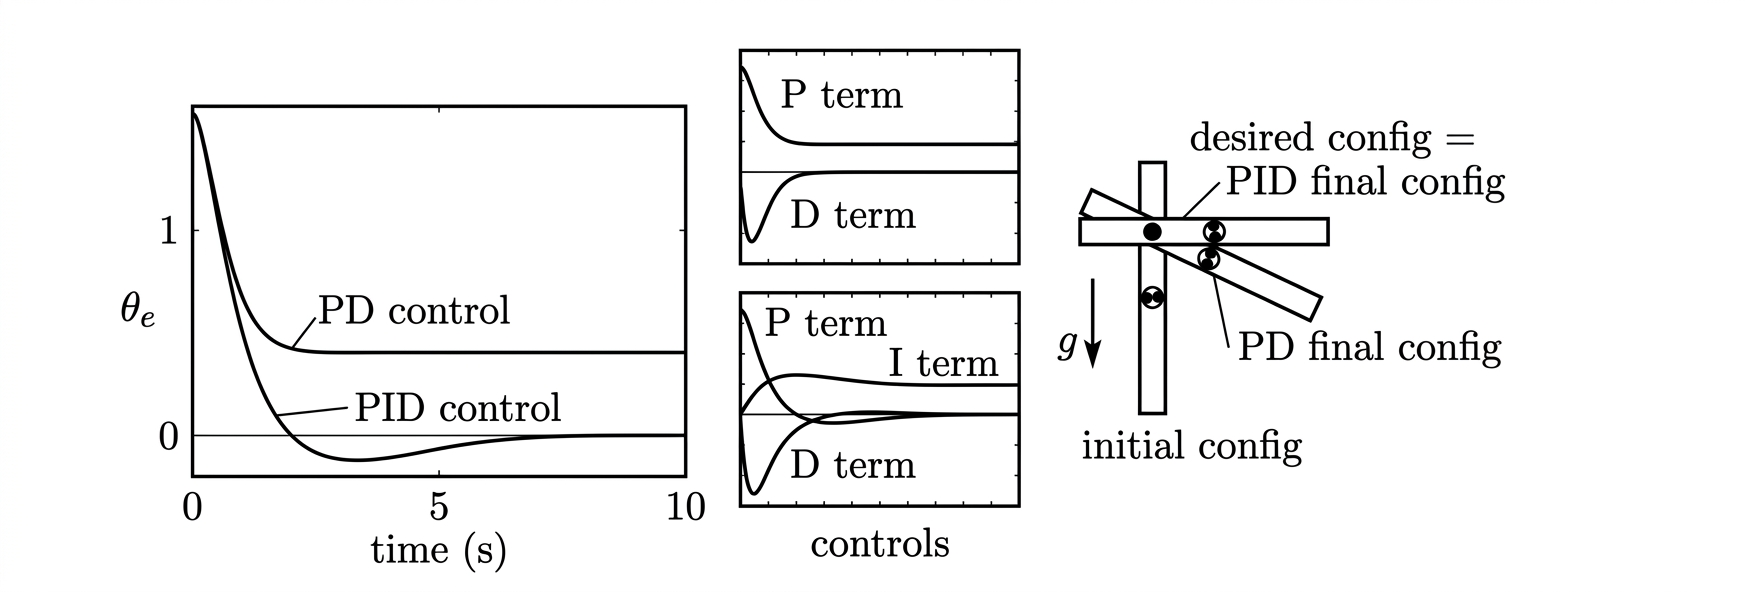
\includegraphics[width=0.8\linewidth]{img/pid.png}
    \begin{flushleft}
    \textit{Note. Adapted from \parencite{lynch2017modern}} 
    \end{flushleft}
\end{figure}

In certain applications, such as real-time drone attitude stabilization, a Proportional-Derivative (PD) controller may be sufficient. This is because the primary objective in such scenarios is to achieve fast and stable responses rather than eliminating steady-state error entirely. Moreover, user-controlled inputs, such as joystick commands, do not necessarily require exact convergence to a fixed reference value. As a result, omitting the integral component can simplify the control system and improve responsiveness.


